\subsection{Training}
\label{subsec:training}

% Optimiser: Adam w/ learning rate 1e-3
% For our experiments we consider training both on single-image datasets and on the full dataset. The single-image datasets are created by manually selecting an image from the full dataset that best represents a specific visual effect, like graininess or colour cast. For such datasets, we train and evaluate the model on the same image to ensure that the model learns the desired effect. The full dataset is used to train a model that can generalize to a wide range of visual effects, and is split into a training, validation and test split according to the guidelines in Section~\ref{subsec:training}.

% Patched training
Beginning with the simplest task, we explored the ability of our architecture to learn Cinestill 800T grain patterns on small patches of a singular image -- testing its ability to overfit and memorize grain patterns. Observing which loss functions and combinations of loss functions proved most effective, we then expanded to training on the full dataset, evaluating the model's ability to generalize to unseen images.


\begin{figure}
  \centering
  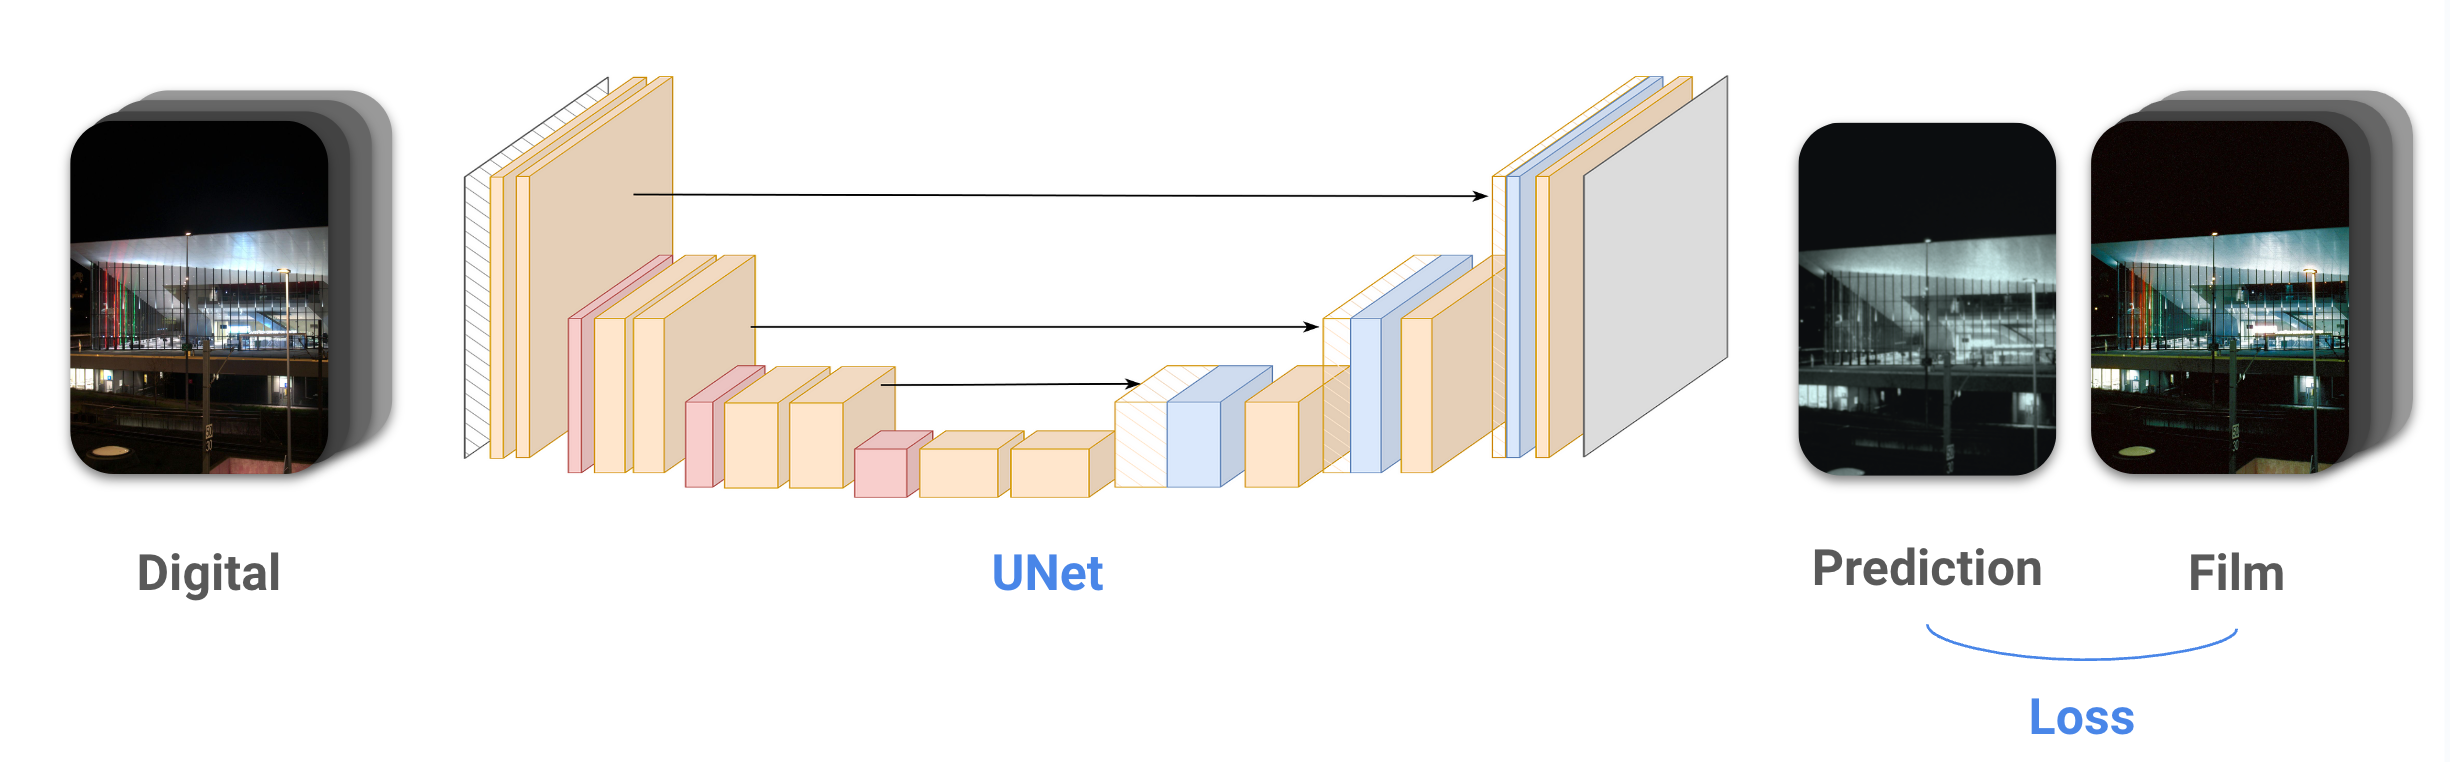
\includegraphics[width=0.9\textwidth]{figures/training-overview.png}
  \caption{\textbf{Training Overview.} We train our model on a dataset of paired digital-film images. The dataset is split into a training, validation and test set. The model is trained using the Adam optimizer with a learning rate of $1e-3$. We use a patched training approach, where the images are divided into patches of size $256 \times 256$ and the model is trained on these patches.}
  \label{fig:training-overview}
\end{figure}

% Training on single-image datasets

% \begin{figure}
%     \centering
%     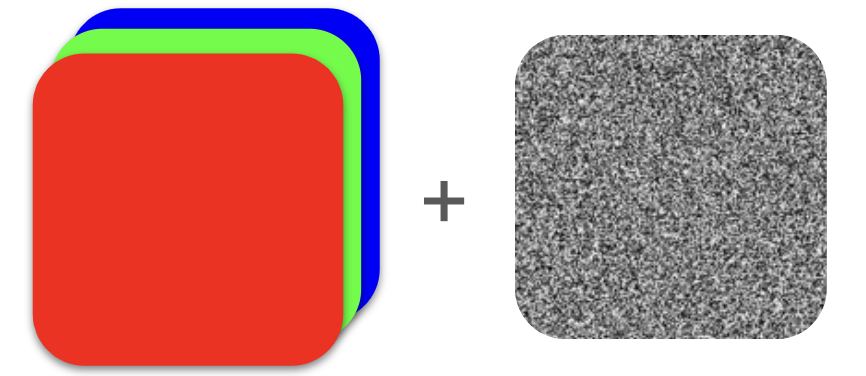
\includegraphics[width=0.5\textwidth]{figures/RGBnoise.png}
%     \caption{\textbf{Original RGB Channels, Random Noise Channel}}
%     \label{fig:random-noise-channel}
% \end{figure}


% Adding noise channel
From single-image experiments with MSE and VGG loss, we observed that the model was able to learn grain patterns on small patches of a single image. However, the grain patterns of small patches were memorized by the model and such patterns were not consistent across the dataset, and so the model struggled to generalize to unseen images.

% TODO go into more detail about single-image experiments with different loss functions

To aid our model's ability to learn noise patterns, we seed our models with an extra random noise channel. We vary the distribution from which the random seed noise is drawn using \textcolor{red}{Gaussian and uniform samples}.


% Number of patches (instead of epochs)
% Batch size relatively small at 4